\section{Experimentation}
\label{sec:experiments}

In this section we examine the properties of \SCAMPLON{} and compare them to
properties of \CYCLON{}, a state-of-the-art cyclic peer sampling service.  As
\CYCLON{} uses fixed-sized partial views, we must predefine its partial view
size $c$.  As shown by Erd{\H o}s and R{\' e}nyi\cite{erdos1959random} random
graphs with less than $(|\mathcal{N}|*\ln|\mathcal{N}|)$ connections are likely
to partition - which is not desired for random peer sampling services.  We want
\CYCLON{} to be optimal for a network size of 1000 peers so we set the partial
view size to $c=7\approx \ln{1000}$ while in each cycle we exchange $l=3$
peers.  We call \CYCLON{} undersized when $\ln{|\mathcal{N}}| > c$, oversized
when $\ln{|\mathcal{N}|} < c$ and optimal when $\ln{|\mathcal{N}|} \approx c$.
The experiments\footnote{Implementation:
  https://github.com/anonymous/anonymous4now} involve up to 500,000 nodes and
are carried out on \PEERSIM{} \cite{peersim}, a simulator for peer-to-peer
networks.  We define a cycle as $\Delta t$ in which each peer has executed its
active protocol once.

We inspect three properties characteristic for random graphs, the \emph{average
  shortest path length}, the \emph{average clustering coefficient}, and
\emph{the partial view size distribution}. Additionally, we investigate on
\emph{robustness to random failures}.

%%\subsection{Clustering coefficient}

\begin{figure}
  \centering
  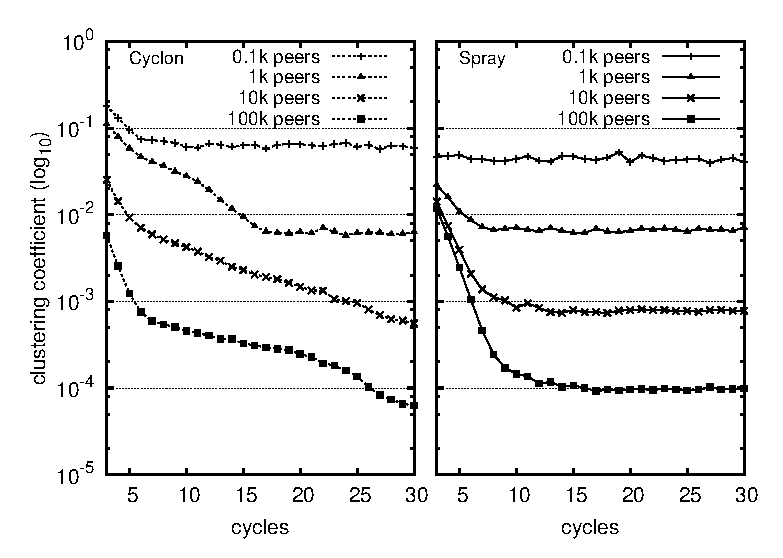
\includegraphics[width=0.49\textwidth]{img/cluster.eps}
  \caption{\label{fig:clustering}Clustering coefficient}
\end{figure}

\ \\
\begin{asparadesc}
\item[Objective:] We want to evaluate to what degree \SCAMPLON{} generates
  clusters in the overlay.  To satisfy the random peer sampling objective it is
  desired that the network has few clusters, thus has a sufficiently low
  clustering coefficient.  This is important for various reasons: first: highly
  clustered networks show poor load-balancing when messages are broadcast as
  peers have a high chance of receiving a message multiple times through their
  neighbors; and second: A network consisting of poorly connected clusters is
  less robust regarding peers failing or simply leaving the overlay to
  disconnect the graph.
\item[Description:] The average clustering coefficient $\overline{C}$ measures
  the connectivity of each peer's neighborhood in the network.
  \begin{equation}
    \overline{C} = {1\over |\mathcal{N}|}\sum\limits_{x\in\mathcal{N}}C_x
  \end{equation}
  where $C_x$ is the local clustering coefficient of Peer $p_x$. The higher the
  coefficient, the more likely the network contains cliques.  The experiments
  involve 100, 1000, 10000 and 100000 peers.
\item[Results:] Figure \ref{fig:clustering} shows that \SCAMPLON{} converges
  much quicker than \CYCLON{}.  Furthermore, oversized \CYCLON{} converges to a
  higher value than \SCAMPLON while it converges to a lower one when
  undersized.
\item[Reasons:] The experiments yield the expected results: \SCAMPLON{}
  converges much quicker as it is not constraint by a fixed, artificial barrier
  $l$.  On the other hand, \CYCLON{} yields a lower clustering coefficient on
  convergence when undersized.  This can be explained by the fact that peers in
  an undersized \CYCLON{} overlay have less connections and thus have a lower
  probability of forming cliques.  This, however, makes it more vulnerable to
  node failure and churn.
\end{asparadesc}

%% \subsection{Average path length}

\begin{figure}
  \centering
  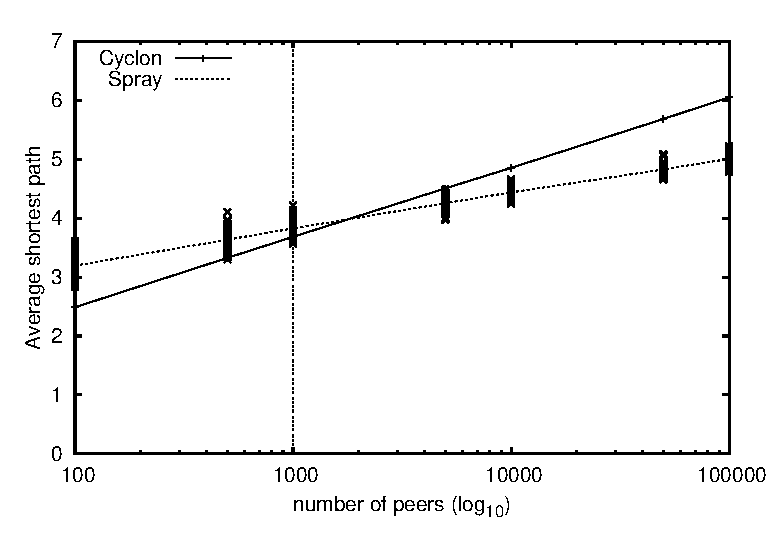
\includegraphics[width=0.49\textwidth]{img/avgpath.eps}
  \caption{\label{fig:avgpath}Average shortest path}
\end{figure}

\ \\
\begin{asparadesc}
\item[Objective:] In this experiment we examine the shortest path length that
  peers have to all other nodes in the network.  For messages to disseminate
  quickly into the network it is crucial that the shortest path to other peers
  is, in fact, short.
\item[Description:] The average path length is the average of the shortest path
  length between peers in the graph. It counts the minimum number of hops to
  reach a peer from another given peer.  For performance reasons, we select a
  subset of 7 nodes, calculated their average shortest path and averaged it.
\item[Results:] Figure~\ref{fig:avgpath} suggests that \CYCLON{}, when
  oversized, yield a shorter average path length then \SCAMPLON{} but quickly
  after its optimum partial view size is exceeded \SCAMPLON{} yields a shorter
  path.
\item[Reasons:] While oversized \CYCLON{} is much better connected into the
  graph and thus yields a lower average path length then \SCAMPLON{}, as soon
  as it is undersized, \SCAMPLON{} is, thanks to bigger partial views, better
  connected into the graph.
\end{asparadesc}

%%\subsection{Partial view size distribution}

\begin{figure}
  \centering
  \includegraphics[width=0.49\textwidth]{img/histo.eps}
  \caption{\label{fig:histo}In-degree distribution}
\end{figure}

\ \\
\begin{asparadesc}
\item[Objective:] As the degree distribution shows the existence of both,
  weakly connected peers as well as strongly connected hubs, it helps to
  analyse the robustness of the overlay when failure is present.  Additionally,
  it indicates how well-distributed links in the network are, which, in turn,
  indicates the resource usage across peers.
\item[Description:] As the overlay can be represented as a directed graph we
  distinguish between out-degree , determining to how many other nodes a peer
  points, and the in-degree, determining from how many other peers a peer is
  referenced.  We concentrate on the in-degree for better comparison as in
  \CYCLON{} the out-degree is fixed ($c$).
\item[Results:] Figure~\ref{fig:histo} shows the in-degree distribution of
  \CYCLON{} and \SCAMPLON{}.  In \CYCLON{} the number of peers in the overlay
  has no influence on the degree distribution always gathers around the
  selected partial view size $c$.  In \SCAMPLON{}, however, the degree
  distribution logarithmically depends on the network size and grows with the
  network.
\item[Reasons:] \CYCLON{}'s fixed partial view size accounts for its rigid
  behavior.  In \SCAMPLON{} the distribution is much more fluid...
\end{asparadesc}

%% \subsection{Churn}
\ \\
\begin{asparadesc}
\item[Objective:] 
\item[Description:] 
\item[Results:]
\item[Reasons:]
\end{asparadesc}

%%\subsection{Resilience to failure}

\begin{figure}
  \centering
  \includegraphics[width=0.49\textwidth]{img/resilience.eps}
  \caption{\label{fig:resilience}Resilience to massive failure}
\end{figure}

\label{subsec:resilience}

\begin{algorithm}

\small
\algrenewcommand{\algorithmiccomment}[1]{\hskip2em$\rhd$ #1}

\newcommand{\comment}[1]{$\rhd$ #1}

\algblockdefx[initially]{initially}{endInitially}
  [0] {\textbf{INITIALLY:}}

\algblockdefx[pas]{pas}{endPas}
  [0] {\textbf{EVENTS:}}

\newcommand{\LINEFOR}[2]{%
  \algorithmicfor\ {#1}\ \algorithmicdo\ {#2} %
  }

\newcommand{\LINEIFTHEN}[2]{%
  \algorithmicif\ {#1}\ \algorithmicthen\ {#2} %
  }

\newcommand{\INDSTATE}[1][1]{\State\hspace{\algorithmicindent}}

\begin{algorithmic}[1]
  \Statex
  \initially
  \State $\mathcal{I}$ \hfill 
  \comment{set of peers targeting us ($p$) in their partial view}
  \endInitially

  \pas
    \Function{unSubscribe}{\ }
    \For{$i\leftarrow 0$ \textbf{to} $min(|\mathcal{P}|,\, |\mathcal{P}|-c-1)$}
    \State \textbf{let} $n,\, age \leftarrow \mathcal{P}[i]$;
    \State $sendTo( \mathcal{I}[\,i\%|\mathcal{I}|\,],\, 'unSubs',\, n)$;
    \EndFor
    \EndFunction
    \Statex
    \Function{onUnSubs}{$o, \, n$} 
    \hfill \comment{$o$: origin; $n$: neighbor to add}
    \State $\mathcal{P}\leftarrow (\mathcal{P}\setminus o)
    \uplus\{\langle n,\,0\rangle\}$;
    \EndFunction
  \endPas
\end{algorithmic}

\caption{\label{algo:unsubscription}Unsubscription protocol from
  \SCAMP{}~\cite{ganesh2003peer}}
\end{algorithm}

\ \\
\begin{asparadesc}
\item[Objective:] 
\item[Description:] Algorithm~\ref{algo:unsubscription} shows the
  unsubscription protocol which guarantees connectedness (WITH HIGH PROBA?)
  upon the assumption that an \emph{in view} $\mathcal{I}$ is maintained
  (cf. Line~\ref{line:inview}) along with bidirectional connections. The set of
  peers which have a particular peer in their partial view populate the
  latter's in view. When a peer leaves, it actively contributes to repair the
  network by acting like a bridge between its in view $\mathcal{I}$ and its
  partial view $\mathcal{P}$. As consequence, the neigbors from $\mathcal{I}$
  add each peer from the leaving peer's partial view in their own partial view.
  Except for one peer (cf. Line~\ref{line:bridge}), it guarantees that these
  peers stay connected, i.e., that at least one partial view references them.
\item[Results:]
\item[Reasons:]
\end{asparadesc}

%% \subsection{Synthesis}

%%% Local Variables:
%%% mode: latex
%%% TeX-master: "../paper"
%%% End:
